\documentclass{standalone}

\usepackage[euler-digits]{eulervm}

\usepackage{tikz}
\tikzset{every node/.style={circle,draw,minimum size=6mm,inner sep=0pt}}
\tikzset{t/.style={rectangle}}
\tikzset{l/.style={above,draw=none,font=\small}}
\tikzset{a/.style={red,very thick,->,>=latex}}
\begin{document}
    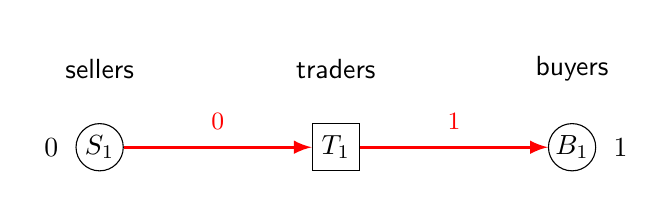
\begin{tikzpicture}[font=\sffamily]
        \node[draw=none] (S) at (-3,5) {sellers};
        \node[draw=none] (B) at (3,5) {buyers};
        \node[draw=none] (T) at (0,5) {traders};
      \node[label=left:{$0$}] (S1) at (-3,4) {$S_1$}; 
      \node[label=right:{$1$}] (B1) at (3,4) {$B_1$}; 
      \node[t] (T1) at (0,4) {$T_1$}; 
      \draw[a] (S1) -- node[l] {$0$} (T1);
      \draw[a] (T1) -- node[l] {$1$} (B1);
    \end{tikzpicture}
\end{document}
